\documentclass[aspectratio=169,17pt]{beamer}

\usetheme{Madrid}
\usecolortheme{default}
\setbeamertemplate{navigation symbols}{}
\setbeamertemplate{footline}[frame number]

\usepackage[T1]{fontenc}
\usepackage[utf8]{inputenc}
\usepackage[english]{babel}
\usepackage{times}
\usepackage{booktabs}
\usepackage{tikz}
\usepackage{amsmath}
\usetikzlibrary{arrows.meta,positioning,shapes.geometric,fit}

\definecolor{uspblue}{RGB}{0,63,122}
\definecolor{usplight}{RGB}{232,241,250}
\setbeamercolor{structure}{fg=uspblue}
\setbeamercolor{title}{fg=white,bg=uspblue}
\setbeamercolor{frametitle}{fg=white,bg=uspblue}
\setbeamercolor{block title}{fg=white,bg=uspblue}
\setbeamercolor{block body}{bg=usplight}
\setbeamercolor{alerted text}{fg=uspblue}

\title[Can AI Sentiment Improve Forex Trading?]{Can AI-Driven Sentiment Improve Forex Trading?}
\author[Wellington Souza]{Wellington Souza}
\institute[ICMC/USP]{MBA in Artificial Intelligence and Big Data \\ ICMC, University of S\~ao Paulo}
\date{S\~ao Carlos, 2026}

\begin{document}

\begin{frame}
  \titlepage
  \vspace{-0.6cm}
  \begin{center}
    \small Advisor: Prof.\ Dr.\ Carolina Toledo Ferraz
  \end{center}
\end{frame}

\begin{frame}{Introduction and Motivation}
  \begin{itemize}
    \item Forex reacts to price, liquidity, macroeconomic news and geopolitical shocks.
    \item Price-only strategies can miss part of that information set.
    \item This work tests whether news-derived event features add predictive value.
  \end{itemize}
\end{frame}

\begin{frame}{Objective and Research Question}
  \small
  \begin{itemize}
    \item \textbf{Objective}: design and evaluate a hybrid Forex strategy using price signals and GDELT event intensity.
    \item \textbf{Question}: does the event family improve performance over a price-only baseline?
    \item Execution: GDELT event intensity; text sentiment was not evaluated.
    \item The answer is based on paired comparison, registered configurations and reproduced results.
  \end{itemize}
\end{frame}

\begin{frame}{Theoretical Background}
  \begin{itemize}
    \item Forex market structure, transaction costs and out-of-sample evaluation.
    \item Financial machine learning and overfitting risk in backtests.
    \item Financial NLP as motivation; executed experiments use coded events, not article-level sentiment.
  \end{itemize}
\end{frame}

\begin{frame}{Methodology: Executed Pipeline}
  \centering
  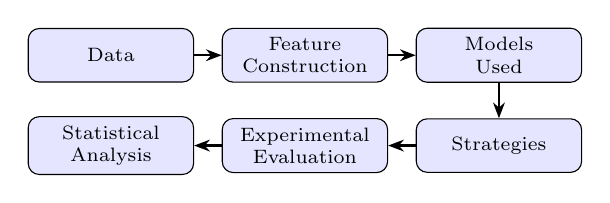
\begin{tikzpicture}[
    node distance=0.45cm and 0.35cm,
    pipebox/.style={draw, rounded corners, fill=blue!10, minimum width=2.1cm, minimum height=0.68cm, align=center, font=\scriptsize},
    arrow/.style={-{Stealth[length=2mm]}, thick}
  ]
  \node[pipebox] (data) {Data};
  \node[pipebox, right=of data] (features) {Feature\\Construction};
  \node[pipebox, right=of features] (models) {Models\\Used};
  \node[pipebox, below=of models] (strategies) {Strategies};
  \node[pipebox, left=of strategies] (evaluation) {Experimental\\Evaluation};
  \node[pipebox, left=of evaluation] (stats) {Statistical\\Analysis};
  \draw[arrow] (data) -- (features);
  \draw[arrow] (features) -- (models);
  \draw[arrow] (models) -- (strategies);
  \draw[arrow] (strategies) -- (evaluation);
  \draw[arrow] (evaluation) -- (stats);
  \end{tikzpicture}
\end{frame}

\begin{frame}{Methodology: Evaluation}
  \begin{itemize}
    \item Three price-family models in the baseline; the hybrid adds one event-family model.
    \item Logistic meta-learner receives only family-model probabilities.
    \item Both strategies run under the same execution model, costs and controls.
  \end{itemize}
\end{frame}

\begin{frame}{Results and Discussion}
  \begin{columns}[T]
    \column{0.48\textwidth}
    \centering
    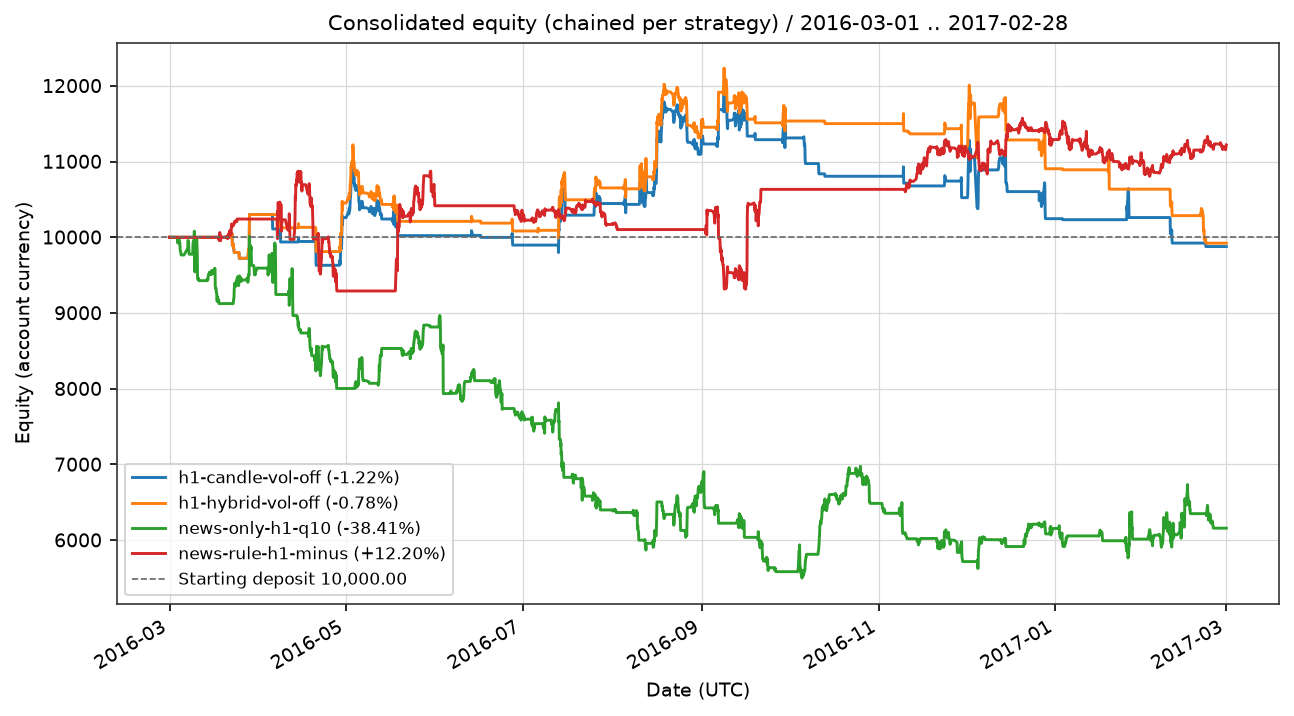
\includegraphics[width=0.95\textwidth]{img/equity-trading-year-h1.png}\\
    \tiny March 2016 -- Feb 2017, EUR/USD (window registered before simulation).
    \column{0.48\textwidth}
    \small
    \begin{itemize}
      \item \alert{Paired hybrid vs.\ baseline difference not significant} ($p=0.149$).
      \item Main result reproduced with the same numbers.
      \item Positive cell = drift (always-short control, $p=0.92$).
    \end{itemize}
  \end{columns}
\end{frame}

\begin{frame}{Discussion of Negative Results}
  \begin{itemize}
    \item A positive return in one cell did not imply predictive ability.
    \item Thresholds calibrated on one month did not survive a level shift.
    \item The observed news signal was short-horizon, while the exit rule held positions for days.
  \end{itemize}
\end{frame}

\begin{frame}{Complementary Results}
  \begin{itemize}
    \item \textbf{Adaptive retraining}: frozen policy lost $97.8\%$ over the year; the other policies remain future work.
    \item \textbf{Candlestick catalog}: the single positive pattern was indistinguishable from chance after multiple-comparisons control.
    \item \textbf{News + candlestick}: the agreement gate had no news-side direction to confirm the pattern.
  \end{itemize}
\end{frame}

\begin{frame}{News and the Positive Pattern}
  \begin{columns}[T]
    \column{0.54\textwidth}
    \centering
    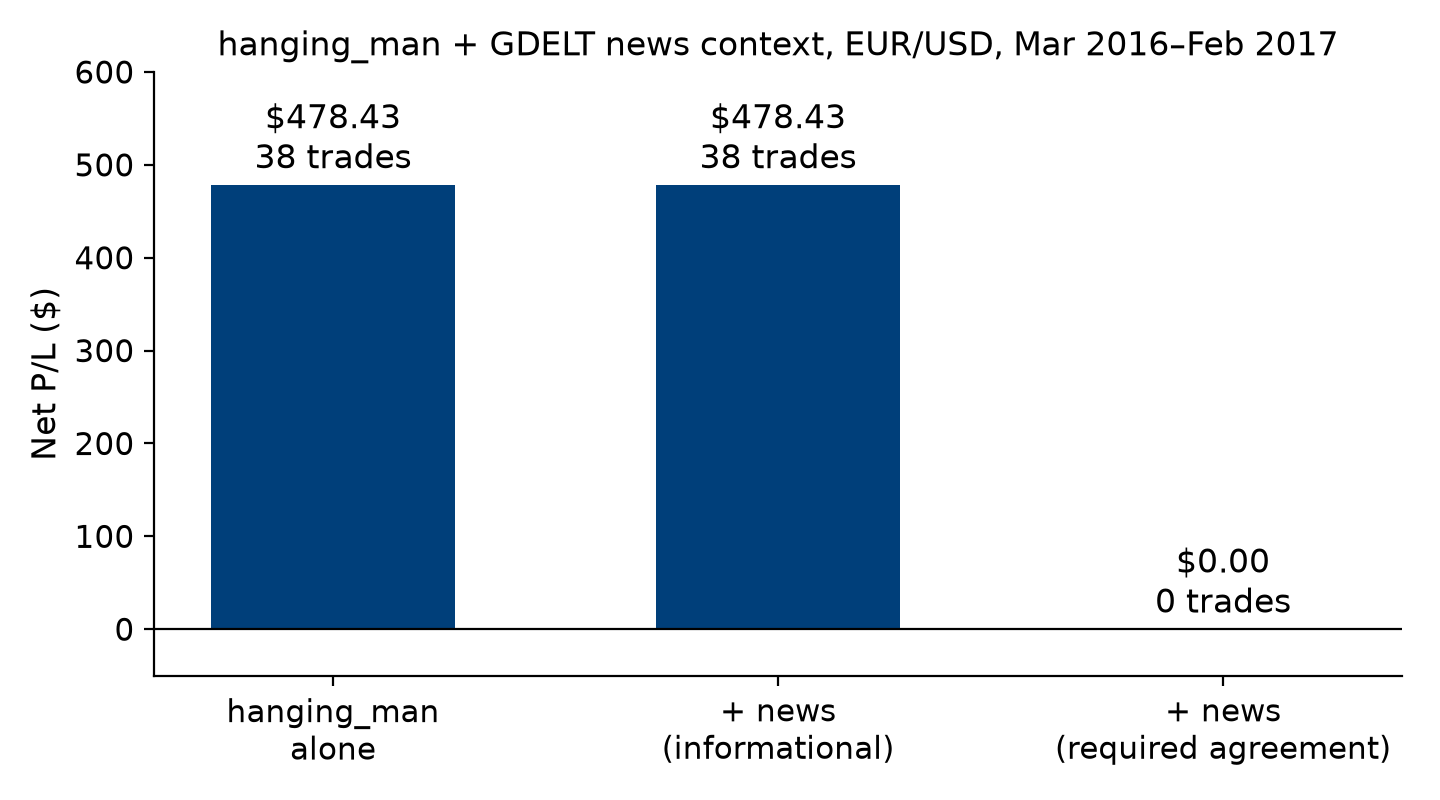
\includegraphics[width=\textwidth]{img/candlestick-news-combination.png}
    \column{0.42\textwidth}
    \small
    \begin{itemize}
      \item Informational news mode: identical trades.
      \item Agreement required: zero trades.
      \item F4 abstained on all eligible bars; no active disagreement was observed.
    \end{itemize}
  \end{columns}
\end{frame}

\begin{frame}{Conclusion}
  \begin{itemize}
    \item In the tested configuration, the answer to the research question is negative.
    \item The main scientific lesson is that apparent profit can reflect drift rather than prediction.
    \item The empirical contribution is an interpretable, reproducible and audited negative result.
    \item The technical contribution is the reusable pipeline, replay and audit-trail infrastructure.
  \end{itemize}
\end{frame}

\begin{frame}{Limitations and Future Work}
  \begin{itemize}
    \item Limitations: one main window, one currency pair and hand-picked thresholds never fitted on held-out data.
    \item Planned components, such as text sentiment, full article text and additional sources, were not evaluated.
    \item Future work: adaptive retraining, confluence chain, intermarket features and additional pairs.
  \end{itemize}
\end{frame}

\begin{frame}
  \centering
  {\Large Thank you. Questions?}
\end{frame}

\end{document}
